\section{Results}


\subsection{Effect of spatial structure in PD and HD games}
In our first simulation experiment, we compared the effect of spatial structure on the persistence of cooperators in the PD and HD games.





The regression shows a significant correlation between estimates and the attitude statement (figure \ref{fig: task1_4plot}): The higher the estimated number of refugees, the more likely people oppose hosting more refugees.



\begin{figure}
	\centering 
	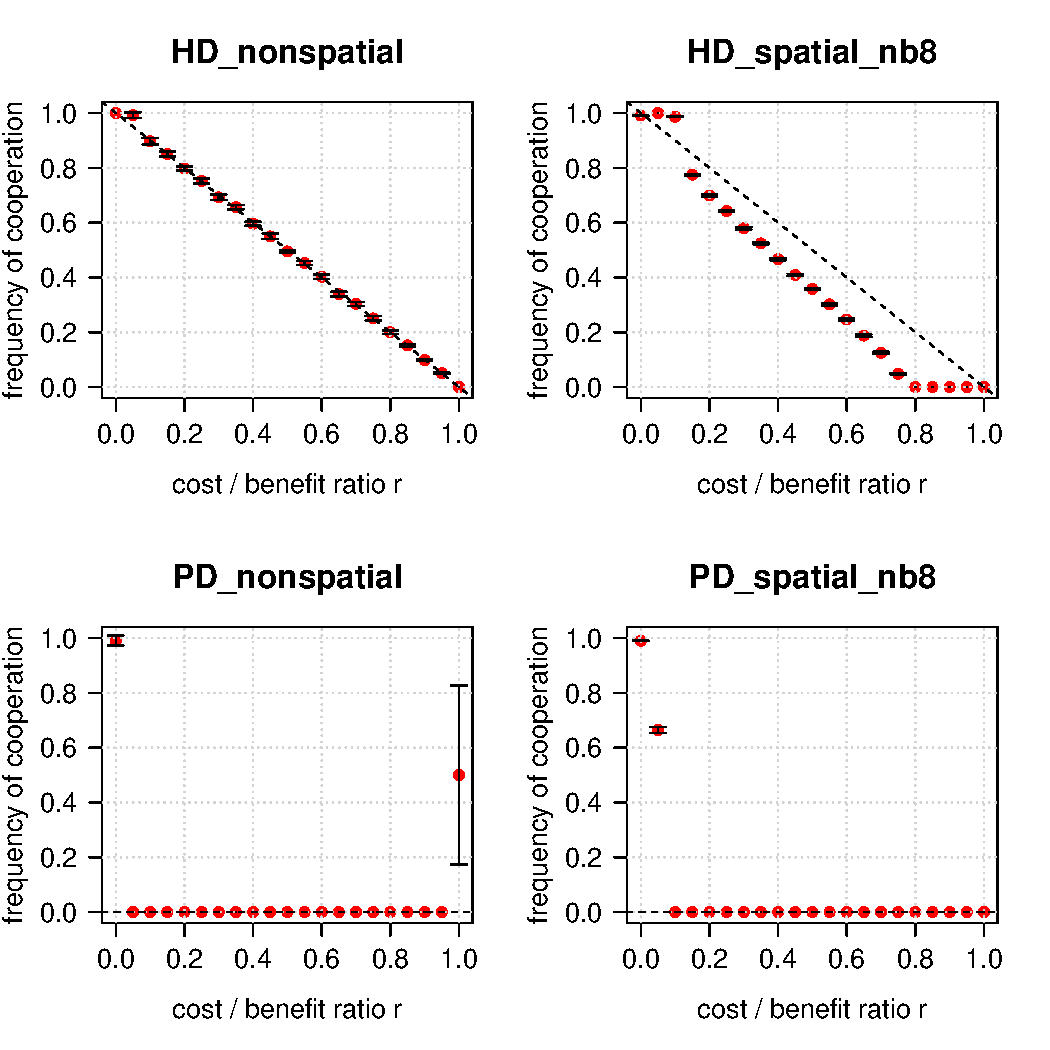
\includegraphics[width=9.5cm]{task1_4plot}
	\caption{Comparison of HD and PD game simulations, both with and without spatial structure.  \textbf{[ t = 5000, i = 10 ]} }\label{fig: task1_4plot}
\end{figure}


\begin{figure}
	\centering 
	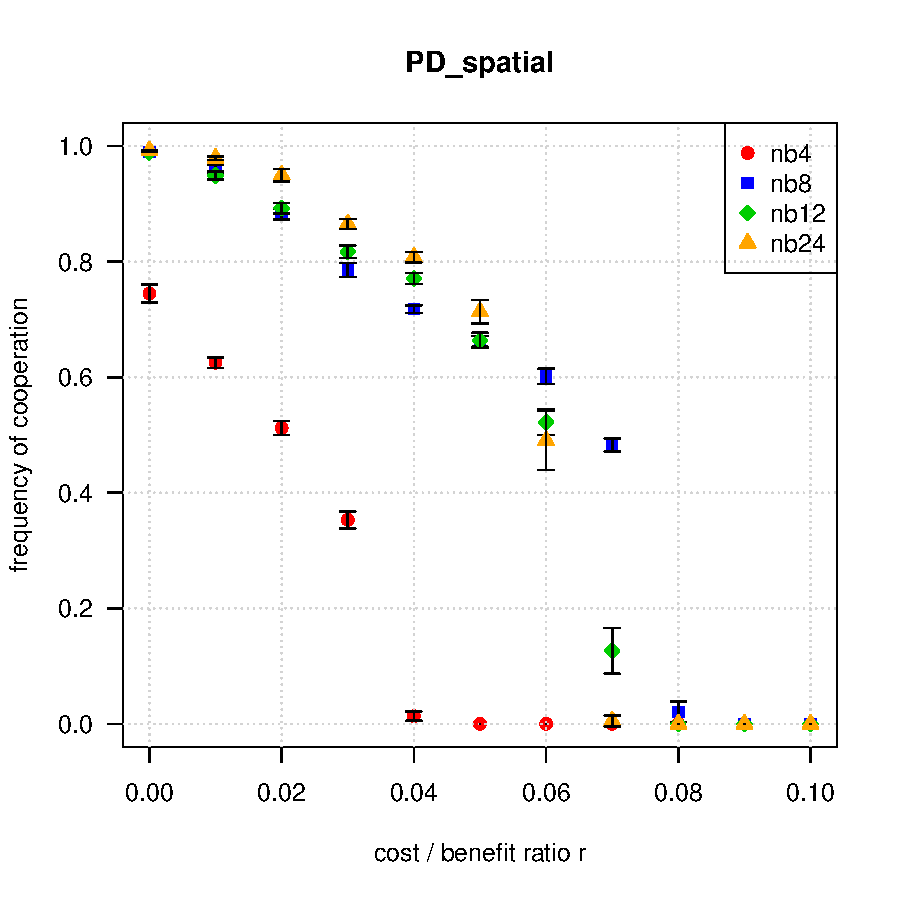
\includegraphics[width=9.5cm]{task2_multiplot}
	\caption{Spatial PD game simulations with different neighbourhood sizes.  \textbf{[ t = 5000, i = 10 ]} }\label{fig: task2_multiplot}
\end{figure}

\begin{figure}[H]
	\centering 
	\includegraphics[width=7cm]{ModelPlot}
	\caption{Attitude towards refugees in dependence of estimated numbers. Blue = regression line}\label{fig: ModelPlot}
\end{figure}


\subsection{Effect of neighbourhood size}


\textbf{HD games} 


\textbf{PD games} 

\textbf{Place:} Unlike with the other variables, the place where interviews were conducted had a significant influence on the attitudes expressed. The ANOVA we returned a p-value of 0.0386.
In Vauban and on campus, people were more positive towards refugees than in the hiking area or at the technical faculty (see figure \ref{fig: Place}).

\begin{figure}
	\centering 
	\includegraphics[width=7cm]{Place}
	\caption{Attitudes towards refugees at different places}\label{fig: Place}
\end{figure}


\subsection{Effect of mixed strategies}

